% =====================================================================
%  Capítulo 4 — Cómo actuar
% =====================================================================
\chapter{Cómo actuar}
\citacap{Saber no es suficiente; debemos aplicar. Querer no es suficiente; debemos hacer.}{Johann Wolfgang von Goethe}

Los principios fundamentales dictan que toda respuesta de defensa personal debe ser:

\begin{itemize}
  \item Rápida
  \item Fuerte
  \item Natural
  \item Directa
\end{itemize}

La idea básica consiste en ocuparse primero de la amenaza inmediata (por ejemplo, un estrangulamiento), impedir que el agresor vuelva a atacar y, solo si es imprescindible, neutralizarle. Se hace énfasis en quitarle la iniciativa.

Es importante \textbf{anticiparse}: todo gesto físico tiene un \enquote{armado}, una \enquote{trayectoria} y un \enquote{impacto}, y con entrenamiento puede verse e interceptarse.

\section{La secuencia en un conflicto}

\begin{enumerate}
  \item \textbf{Cúbrete:} si el objetivo del agresor es pegarte, lo intentará hasta que se canse o algo lo detenga. Interesa cubrir cabeza, cuello y torso. Llevarse un golpe en brazos o piernas siempre será mejor que en la sien, la garganta o las costillas.
  \item \textbf{Anula su visión:} lanzando objetos a la cara del agresor, usando nuestras manos y dedos, escupiendo a los ojos, etc.
  \item \textbf{Gana tiempo} buscando su desequilibrio: empujón con una o ambas manos.
  \item \textbf{Huye:} correr sí, pero no en cualquier momento ni dirección. Antes del sprint hacia el punto de huida, coloca al agresor en una situación en la que no pueda interceptarte (movimiento obligado). Huye hacia luz, gente y ruido, nunca hacia zonas más aisladas.
\end{enumerate}

\section{Lucha, huida\ldots{} y parálisis: lo que dice la ciencia actual}

Ante un enfrentamiento se libera un torrente hormonal (adrenalina, cortisol) que prepara el organismo para combatir o emprender la fuga: visión en túnel, aumento de pulsaciones, pérdida de motricidad fina. Entrenar bajo estrés (con compañero, protecciones y escenarios) reduce estos efectos y nos enseña a operar con ellos.

Pero la investigación reciente ha confirmado una tercera respuesta involuntaria: la \textbf{inmovilidad tónica} o parálisis. Un estudio sueco con 298 supervivientes de violación \citep{moller2017} encontró que el 70\,\% experimentó inmovilidad significativa durante la agresión. Es una respuesta neurobiológica automática, no una decisión ni una forma de consentimiento. Esto tiene dos consecuencias prácticas: primero, si alguna vez te quedaste paralizada, no fue culpa tuya ni debilidad; segundo, el entrenamiento repetido y realista es precisamente la herramienta que más reduce la probabilidad de quedarse bloqueada, porque da al cerebro respuestas preprogramadas que ejecutar.

\newpage

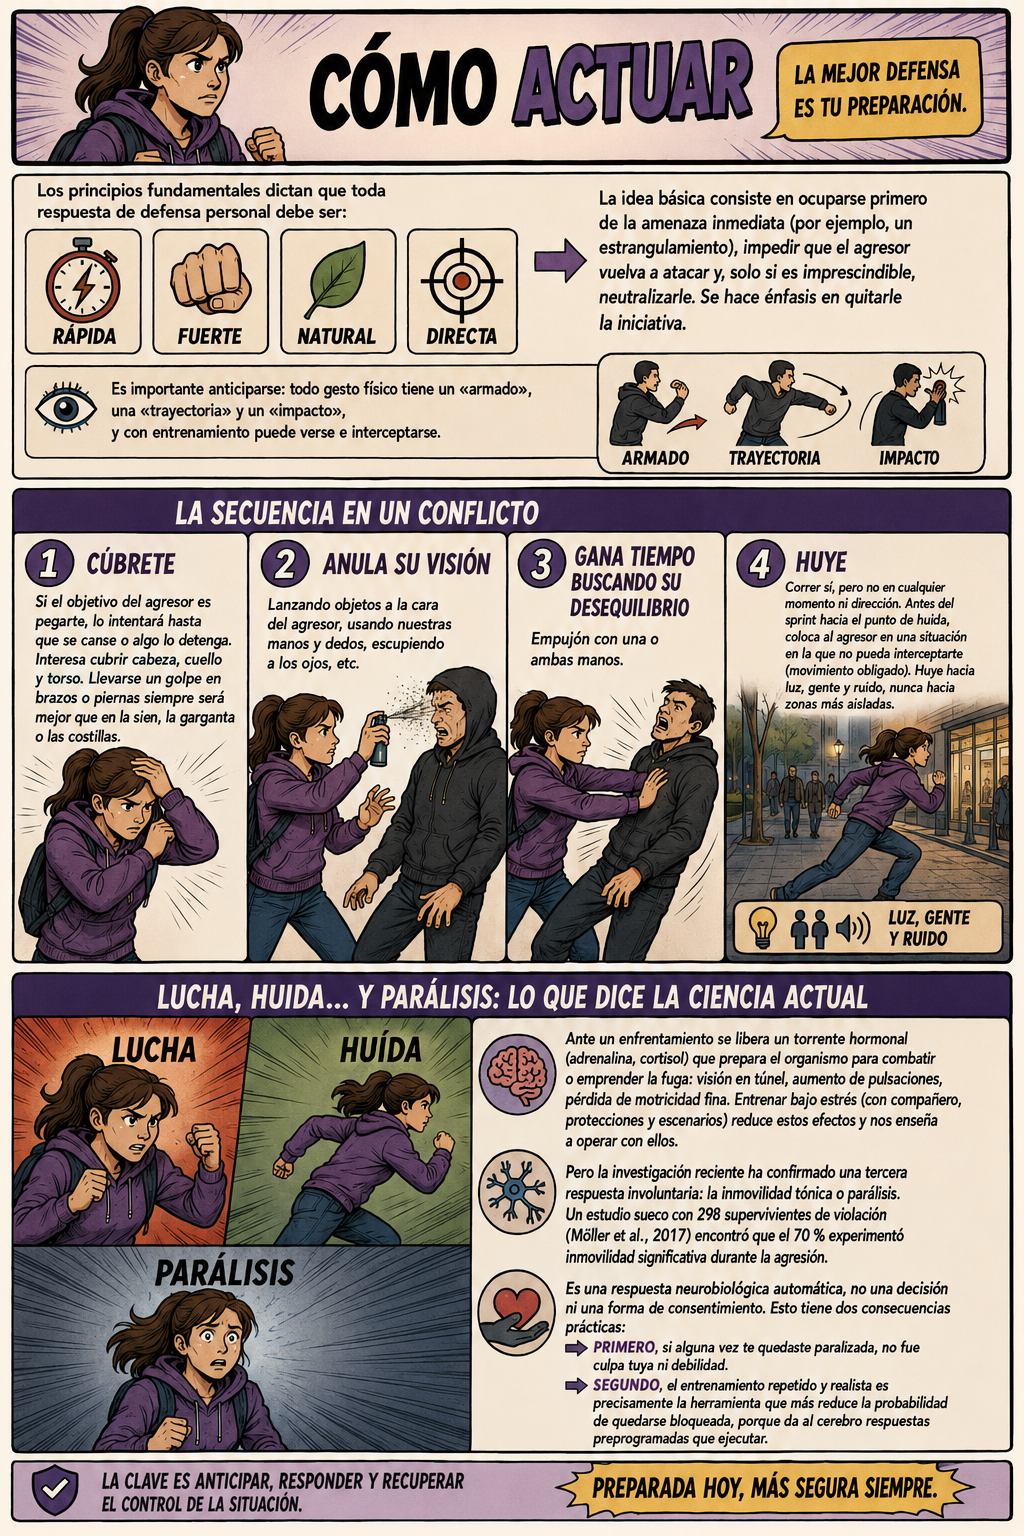
\includegraphics[width=\linewidth]{figures/como-actuar.png}
